\section{CMS Datasets} \label{section:higgs_data}
At CMS, all of the accumulated data is organized in terms of datasets, which can be logically organized into key-value pairs. A key is the name of a dataset, which uniquely identifies it across the rest of the samples (dataset and sample are used interchangeably). At the same time, a key follows a standard naming convention, which allows to quickly resolve the most important characteristics of the actual data it points to. A value, in turn, is a collection of data files that actually constitute the dataset and are used for the analysis.

Generally speaking, the CMS experiment produces two types of datasets: collision and simulation samples. Collision samples correspond to the actual data recorded from proton-proton collisions at the LHC. A typical collision sample name has three parts: stream identifier, timestamp and format of the data stored. Depending on the format, timestamp can either point to the actual period of datataking or the reconstruction date. The CMS assigns descriptive stream identifiers in order to provide an overview of the physical content of the events that go into a dataset. For instance, in this search, only events that have a good quality muon object are considered and a ''SingleMuon'' identifier signals exactly that. Furthermore, datasets could have identifiers like ''SingleElectron'' or ''SinglePhoton'', which would make them respectively contain events with an electron or a photon.

Simulation samples correspond to the data produced by simulating the collisions environment (production processes and consecutive decays) and the response of the CMS detector. The most important use case of the simulation is to provide a modeling baseline with which collisions data will be compared. For the purpose of the search, simulation datasets can be further divided into the signal and background samples. Signal corresponds to the Higgs Boson production processes with its consecutive decay to two muons. Backgrounds, in turn, are basically all of the processes that can produce the same signature, the same final state. A typical unique simulation sample name, similar to collision sample name, has three parts: production process specifier, conditions identifier and the format of the data stored. The first part specifies a label that summarizes the actual production process and the Monte Carlo event generators used to perform the calculations of the Feynman diagrams. Conditions part carries a label to uniquely specify a campaign when a sample is produced, software versions used, and various calibrations and corrections applied.

\subsection{Collision Datasets}
For the purpose of the search, datasets with the total integrated luminosity of 35.9 fb$^{-1}$ of CMS collisions data collected over the course of 2016 datataking campaign are utilized and the full list of these samples is provided in the Table~\ref{table:higgs_data_collisiondatasets}. The signature of the search is the presence of two opposite sign muons in the event, therefore, in order to pick up as many as possible events of interest, the choice for the stream identifier is limited to either ''SingleMuon'' or ''DoubleMuon''. The choice of ''SingleMuon'' is dictated by the fact of having intrinsically higher efficiency of triggering a single muon rather than two muons per a given event. By selecting ''DoubleMuon'' trigger, for this particular search, all the events where only one muon triggers the HLT system would be thrown away. Therefore, considering that dimuon final state has a very low branching fraction for the Higgs Boson, the choice is made not to throw away the events.
\begin{table}[htb]
    \caption{Datasets, used for the search, from proton-proton collisions recorded at the $\sqrt{s}=13$~TeV by CMS at LHC in 2016}
    \label{table:higgs_data_collisiondatasets}
    \begin{center}
        \begin{tabular}{ l  c}
            \hline
            Datasets & Int. Luminosity (fb$^{-1}$)\\
            \hline
            {/SingleMuon/Run2016B-03Feb2017\_ver2-v2/MINIAOD} & 5.788\\
            {/SingleMuon/Run2016C-03Feb2017-v1/MINIAOD} & 2.573\\
            {/SingleMuon/Run2016D-03Feb2017-v1/MINIAOD} & 4.248\\
            {/SingleMuon/Run2016E-03Feb2017-v1/MINIAOD} & 4.009\\
            {/SingleMuon/Run2016F-03Feb2017-v1/MINIAOD} & 3.102\\
            {/SingleMuon/Run2016G-03Feb2017-v1/MINIAOD} & 7.540\\
            {/SingleMuon/Run2016H-03Feb2017\_ver2(3)-v1/MINIAOD} & 8.606\\
            \hline
        \end{tabular}
    \end{center}
\end{table}

\subsection{Signal Datasets}
For the purpose of testing various hypothetical Standard Model Higgs Boson masses, it is crucial to be able to build signal models for each hypothesis. In this analysis, samples with three different hypothetical Higgs Boson masses are used, 120/125/130 GeV, which allows a mass range [120, 130] GeV to be examined. The process of signal model construction and interpolation of parameters as a function of the Higgs Boson mass is discussed further in detail in Section~\ref{section:higgs_signalmodel}. The choice of the mass range is driven by the evidence obtained from searches for the Higgs Boson in other final states, discussed in Section~\ref{section:higgs_run1results}, where observations of a resonance near 125 GeV mass were made. Table~\ref{table:higgs_data_signaldatasets} provides a summary of the CMS signal samples used along with cross section of each production process for the 125 GeV mass hypothesis.
\begin{table}[htb]
    \caption{Standard Model 125 GeV Higgs Boson Signal Datasets for 13 TeV. Dataset names for 120/130 GeV are omitted for brevity. Moriond 2017 conditions are used (omitted the conditions specification for brevity)}
    \label{table:higgs_data_signaldatasets}
        \begin{center}
        \begin{tabular}{ l  c}
            \hline
            Datasets & $\sigma$ (pb)\\
            \hline
            {/GluGlu\_HToMuMu\_M125\_13TeV\_powheg\_pythia8} & 48.58\\
            {/VBF\_HToMuMu\_M125\_13TeV\_powheg\_pythia8} & 3.782\\
            {/WMinusH\_HToMuMu\_M125\_13TeV\_powheg\_pythia8} & 0.5331\\
            {/WPlusH\_HToMuMu\_M125\_13TeV\_powheg\_pythia8} & 0.851\\
            {/ZH\_HToMuMu\_M125\_13TeV\_powheg\_pythia8} & 0.8839 \\
            \hline
        \end{tabular}
        \end{center}
\end{table}
The Higgs signal production processes considered in this search are gluon
fusion (ggH), vector boson fusion (VBF), Higgsstrahlung (VH). Production in
association with top quarks (\ttH) has been generated privately. The Higgs MC samples are generated using {\sc POWHEG}~\cite{Nason:2004rx}.

\subsection{Background Datasets}
As it has already been stated, background processes are the processes that result in the same final state (at least two muons in the event) as the Higgs Boson samples considered. For this analysis, all the processes that produce two muons in the final state, but not through their coupling to the Higgs field,  are to be considered backgrounds. Table~\ref{table:higgs_data_backgrounddatasets} provides a summary of the most dominant contributions among the background processes. The largest contributor is the Drell-Yan process, which constitutes approximately 90\% of background events, and has a pair of leptons in the final state. The next to leading contributor is the $\mathrm{t\bar{t}}$-production, with subsequent decay of top quarks into lighter bottom quarks and W$^{\pm}$ vector bosons further coupling to 2 fermions. These two mechanisms are responsible for more than 98\% of background events contributing to the dimuon final state.
\begin{table}[htb]
    \caption{Background Datasets. Moriond 2017 conditions have been used (omitted the conditions specification for brevity)}
    \label{table:higgs_data_backgrounddatasets}
    \begin{center}
        \begin{tabular}{ l  c}
            \hline
            Dataset & $\sigma$ (pb)\\
            \hline
            /DYJetsToLL\_M-50\_TuneCUETP8M1\_13TeV-amcatnloFXFX-pythia8 & 5765\\
            /ST\_tW\_top\_5f\_NoFullyHadronicDecays\_13TeV-powheg\_TuneCUETP8M1 & 35.85\\
            /TTJets\_DiLept\_TuneCUETP8M1\_13TeV-madgraphMLM-pythia8 & 85.656\\
            /WJetsToLNu\_TuneCUETP8M1\_13TeV-amcatnloFXFX-pythia8 & 61526.7\\
            /WWTo2L2Nu\_13TeV-powheg-herwigpp & 10.481\\
            /WZTo3LNu\_TuneCUETP8M1\_13TeV-amcatnloFXFX-pythia8 & 4.712\\
            \hline
        \end{tabular}
    \end{center}
\end{table}

Depending on the analysis strategy, the role of background simulation samples can be two-fold. First, they are used for comparison with collisions data, in particular to make sure that dimuon mass is modeled well by the included backgrounds. The idea is to show that physical quantities of interest (dimuon mass, various kinematic variables) are in line with theoretical predictions. It is important to point out that both data and simulated samples will be further subject to exactly same selections, further described in Section~\ref{section:higgs_selections}. Second, background datasets can be directly used for the hypothesis testing and statistical analysis of the presence of the signal in the data. In such a case, it is common to abbreviate this approach as simulation driven, because the simulated background dimuon mass distributions are directly used in the hypothesis testing. Another approach, commonly named data driven, is to build a model, similar to the construction of a signal model and discussed further in Section~\ref{section:higgs_bkgmodel}, that will be fit to the actual data, constrained and used to estimate the background yield.

This analysis follows data driven background estimation approach due to the low statistical power of simulated background samples. In other words, significant bin-to-bin fluctuations are present, especially for the categories with lower statistics, that would result in inadequate extraction of the upper limits. Therefore, the primary use of background datasets is to compare various kinematic variable distributions from data and theoretical predictions. Moreover, as it will be clarified in section~\ref{section:higgs_categorization}, depending on the categorization technique used, background samples will be further used for training a binary classification algorithm for the purpose of signal discrimination.

Single top samples are generated with {\sc POWHEG}, whereas $\mathrm{t\bar{t}}$ samples and the multi-boson samples are generated either with {\sc madgrapgh}~\cite{Alwall:2011uj} or {\sc amc@NLO} (Next to Leading Order)~\cite{amcatnlo}. Spin effects in multi boson processes are simulated using {\sc Madspin}. The parton shower and hadronization processes are modeled by the {\sc Pythia8} generator~\cite{Sjostrand:2007gs} with TuneCUETP8M1.

%The simulated pile up distribution is reweighted to match the observed
%distribution in data for all MC samples.

% \begin{table}[!h]
% \small
% \renewcommand{\arraystretch}{1.5}

% \begin{tabular}{|l||l|c|}
%     \hline \textbf{Dataset} & Run Range & Integrated Luminosity \\
%     \hline  &  & [fb$^{-1}$] \\
%     \hline
%         %% %% Fairly certain ver1-v1 is not used at all (no events in Golden JSON - AWB 13.05.16
%     %% \hline \url{/SingleMuon/Run2016B-03Feb2017_ver1-v1/MINIAOD} & \multirow{2}{*}{272007-275376} & \multirow{2}{*}{5.788} \\ \cline{1-1}
%     %% \url{/SingleMuon/Run2016B-03Feb2017_ver2-v2/MINIAOD} &  &  \\
%         \hline \url{/SingleMuon/Run2016B-03Feb2017_ver2-v2/MINIAOD} & 272007-275376 & 5.788 \\
%     \hline \url{/SingleMuon/Run2016C-03Feb2017-v1/MINIAOD}      & 275657-276283 & 2.573 \\
%     \hline \url{/SingleMuon/Run2016D-03Feb2017-v1/MINIAOD}      & 276315-276811 & 4.248 \\
%     \hline \url{/SingleMuon/Run2016E-03Feb2017-v1/MINIAOD}      & 276831-277420 & 4.009 \\
%     \hline \url{/SingleMuon/Run2016F-03Feb2017-v1/MINIAOD}      & 277772-278808 & 3.102 \\
%         \hline \url{/SingleMuon/Run2016G-03Feb2017-v1/MINIAOD}      & 278820-280385 & 7.540 \\
%     \hline \url{/SingleMuon/Run2016H-03Feb2017_ver2-v1/MINIAOD} & \multirow{2}{*}{280919-284044} & \multirow{2}{*}{8.606} \\ \cline{1-1}
%            \url{/SingleMuon/Run2016H-03Feb2017_ver3-v1/MINIAOD} &                                &                        \\
%     \hline                                                         %% Adds up to 35.866 - i.e. 35.9 fb^-1
%     \hline \multicolumn{3}{|l|}{\textbf{Luminosity mask: \url{Cert_271036-284044_13TeV_23Sep2016ReReco_Collisions16_JSON.txt}}}    \\
% \hline
% \end{tabular}

% \caption{Overview of the single muon data stream collected during the
% proton-proton collisions at $\sqrt{s}=13$~TeV by CMS at LHC in 2016.}
% \label{tab:datasets}
% \end{table}

% \newpage
% \begin{landscape}
% \begin{table}[p]
% \renewcommand{\arraystretch}{1.5}
% \tiny
% \begin{tabular}{|l||c|c|c|}
%   \hline \textbf{Higgs signal MC samples} & Events & Cross section [pb] & Xsec $\times$ BR [fb]  \\
%   %% From Yellow Report 4 (https://arxiv.org/abs/1610.07922), H --> mu-mu branching ratio at 125 GeV = 0.0002176
%   %% ggH = 48.58 pb, VBF = 3.7817 pb, W+H = 0.09426 pb, W-H = 0.05983 pb, ZH = 0.17762 pb, ttH = 0.5071 pb
%   \hline
%   \hline \url{/GluGlu_HToMuMu_M125_13TeV_powheg_pythia8/RunIISummer16MiniAODv2-PUMoriond17_80X_mcRun2_asymptotic_2016_TrancheIV_v6-v1/MINIAODSIM }  &  250000 & 48.58    & 10.571   \\
%   \hline \url{/VBF_HToMuMu_M125_13TeV_powheg_pythia8/RunIISummer16MiniAODv2-PUMoriond17_80X_mcRun2_asymptotic_2016_TrancheIV_v6-v1/MINIAODSIM }     &  249200 &  3.7817  & 0.8229   \\
%   \hline \url{/WPlusH_HToMuMu_M125_13TeV_powheg_pythia8/RunIISummer16MiniAODv2-PUMoriond17_80X_mcRun2_asymptotic_2016_TrancheIV_v6-v1/MINIAODSIM }  &  124547 &  0.09426 & 0.02051  \\
%   \hline \url{/WMinusH_HToMuMu_M125_13TeV_powheg_pythia8/RunIISummer16MiniAODv2-PUMoriond17_80X_mcRun2_asymptotic_2016_TrancheIV_v6-v1/MINIAODSIM } &  125000 &  0.05983 & 0.013019 \\
%   \hline \url{/ZH_HToMuMu_M125_13TeV_powheg_pythia8/RunIISummer16MiniAODv2-PUMoriond17_80X_mcRun2_asymptotic_2016_TrancheIV_v6-v1/MINIAODSIM }      &  249748 &  0.17762 & 0.03865  \\
%   %% \hline \url{/ttHToNonbb_M125_TuneCUETP8M2_ttHtranche3_13TeV-powheg-pythia8/RunIISummer16MiniAODv2-PUMoriond17_80X_mcRun2_asymptotic_2016_TrancheIV_v6-v1/MINIAODSIM } & 3981250 & 0.5071 & 0.11034 \\

% \hline
% \end{tabular}

% \caption{The Higgs signal MC samples were generated with {\sc POWHEG}
% while the parton shower and hadronization processes are modeled by the
% {\sc Phythia8} generator with TuneCUETP8M1.}
% \label{tab:SignalMC}
% \end{table}
% \end{landscape}

% \newpage
% \begin{landscape}
% \begin{table}[p]
% \tiny
% \renewcommand{\arraystretch}{1.2}
% \begin{tabular}{|l||c|c|}
%     \hline \textbf{Background MC} & Events & Cross Section [pb]  \\
%     \hline
%     \hline \multicolumn{3}{|c|}{\textbf{Drell--Yan}}  \\
%     \hline
%     \hline \url{/DYJetsToLL_M-50_TuneCUETP8M1_13TeV-amcatnloFXFX-pythia8/RunIISummer16MiniAODv2-PUMoriond17_80X_mcRun2_asymptotic_2016_TrancheIV_v6_ext2-v1/MINIAODSIM} &  122055388 & 5765  \\
%     \hline \url{/DYToLL_0J_13TeV-amcatnloFXFX-pythia8/RunIISummer16MiniAODv2-PUMoriond17_80X_mcRun2_asymptotic_2016_TrancheIV_v6_ext1-v1/MINIAODSIM} & 49579613  &  4754\\
%     %% \hline \url{/DYToLL_0J_13TeV-amcatnloFXFX-pythia8/RunIISummer16MiniAODv2-PUMoriond17_backup_80X_mcRun2_asymptotic_2016_TrancheIV_v6-v1/MINIAODSIM} & 44253240  &  4754    \\
%     \hline \url{/DYToLL_1J_13TeV-amcatnloFXFX-pythia8/RunIISummer16MiniAODv2-PUMoriond17_80X_mcRun2_asymptotic_2016_TrancheIV_v6_ext1-v1/MINIAODSIM} & 49902571  & 888.9 \\
%     %% \hline \url{/DYToLL_1J_13TeV-amcatnloFXFX-pythia8/RunIISummer16MiniAODv2-PUMoriond17_backup_80X_mcRun2_asymptotic_2016_TrancheIV_v6-v1/MINIAODSIM} & 41597712  & 888.9 \\
%     \hline \url{/DYToLL_2J_13TeV-amcatnloFXFX-pythia8/RunIISummer16MiniAODv2-PUMoriond17_80X_mcRun2_asymptotic_2016_TrancheIV_v6-v2/MINIAODSIM} & 42324802  & 348.8 \\
%     \hline \url{/DYToLL_2J_13TeV-amcatnloFXFX-pythia8/RunIISummer16MiniAODv2-PUMoriond17_80X_mcRun2_asymptotic_2016_TrancheIV_v6_ext1-v1/MINIAODSIM} & 47974554  & 348.8 \\
%     %% \hline \url{/DYJetsToLL_M-100to200_TuneCUETP8M1_13TeV-amcatnloFXFX-pythia8/RunIISummer16MiniAODv2-PUMoriond17_80X_mcRun2_asymptotic_2016_TrancheIV_v6_ext1-v1/MINIAODSIM} &  1083606 &  ??? \\
%     \hline
%     \hline \multicolumn{3}{|c|}{\textbf{SingleTop}}    \\
%     \hline
%     \hline \url{/ST_tW_top_5f_NoFullyHadronicDecays_13TeV-powheg_TuneCUETP8M1/RunIISummer16MiniAODv2-PUMoriond17_80X_mcRun2_asymptotic_2016_TrancheIV_v6-v1/MINIAODSIM} & 5372991  & 35.85 \\
%     \hline \url{/ST_tW_top_5f_NoFullyHadronicDecays_13TeV-powheg_TuneCUETP8M1/RunIISummer16MiniAODv2-PUMoriond17_80X_mcRun2_asymptotic_2016_TrancheIV_v6_ext1-v1/MINIAODSIM} & 3256650  & 35.85 \\
%     \hline \url{/ST_tW_antitop_5f_NoFullyHadronicDecays_13TeV-powheg_TuneCUETP8M1/RunIISummer16MiniAODv2-PUMoriond17_80X_mcRun2_asymptotic_2016_TrancheIV_v6-v1/MINIAODSIM} & 5425134  & 35.85 \\
%     \hline \url{/ST_tW_antitop_5f_NoFullyHadronicDecays_13TeV-powheg_TuneCUETP8M1/RunIISummer16MiniAODv2-PUMoriond17_80X_mcRun2_asymptotic_2016_TrancheIV_v6_ext1-v1/MINIAODSIM} & 3256407 & 35.85 \\
%     \hline
%     \hline \multicolumn{3}{|c|}{\textbf{TopPair}}    \\
%     \hline
%     \hline \url{/TTJets_DiLept_TuneCUETP8M1_13TeV-madgraphMLM-pythia8/RunIISummer16MiniAODv2-PUMoriond17_80X_mcRun2_asymptotic_2016_TrancheIV_v6-v1/MINIAODSIM} & 6094476 & 85.656 \\
%     \hline \url{/TTJets_DiLept_TuneCUETP8M1_13TeV-madgraphMLM-pythia8/RunIISummer16MiniAODv2-PUMoriond17_80X_mcRun2_asymptotic_2016_TrancheIV_v6_ext1-v1/MINIAODSIM} & 24350202  & 85.656 \\
%     \hline \url{/TTJets_Dilept_TuneCUETP8M2T4_13TeV-amcatnloFXFX-pythia8/RunIISummer16MiniAODv2-PUMoriond17_80X_mcRun2_asymptotic_2016_TrancheIV_v6-v1/MINIAODSIM} &  14529280 & 85.656  \\
%     \hline
%     \hline \multicolumn{3}{|c|}{\textbf{DiBoson}}    \\
%     \hline
%     \hline \url{/WWTo2L2Nu_13TeV-powheg/RunIISummer16MiniAODv2-PUMoriond17_80X_mcRun2_asymptotic_2016_TrancheIV_v6-v1/MINIAODSIM } & 1999000  & 12.46  \\
%     \hline \url{/WZTo3LNu_TuneCUETP8M1_13TeV-amcatnloFXFX-pythia8/RunIISummer16MiniAODv2-PUMoriond17_80X_mcRun2_asymptotic_2016_TrancheIV_v6-v1/MINIAODSIM} & 11887464  & 2.113 \\
%     \hline \url{/WZTo2L2Q_13TeV_amcatnloFXFX_madspin_pythia8/RunIISummer16MiniAODv2-PUMoriond17_80X_mcRun2_asymptotic_2016_TrancheIV_v6-v1/MINIAODSIM} & 26517272  &  4.409 \\
%     \hline \url{/ZZTo2L2Nu_13TeV_powheg_pythia8/RunIISummer16MiniAODv2-PUMoriond17_80X_mcRun2_asymptotic_2016_TrancheIV_v6-v1/MINIAODSIM} & 8842475  & 0.564  \\
%     \hline \url{/ZZTo2L2Q_13TeV_amcatnloFXFX_madspin_pythia8/RunIISummer16MiniAODv2-PUMoriond17_80X_mcRun2_asymptotic_2016_TrancheIV_v6-v1/MINIAODSIM} & 15345572  & 3.22 \\
%     \hline \url{/ZZTo4L_13TeV-amcatnloFXFX-pythia8/RunIISummer16MiniAODv2-PUMoriond17_80X_mcRun2_asymptotic_2016_TrancheIV_v6_ext1-v1/MINIAODSIM} &  10709784 & 1.212  \\
%     \hline
%     \hline \multicolumn{3}{|c|}{\textbf{TriBoson}}   \\
%     \hline
%     \hline \url{/WWW_4F_TuneCUETP8M1_13TeV-amcatnlo-pythia8/RunIISummer16MiniAODv2-PUMoriond17_80X_mcRun2_asymptotic_2016_TrancheIV_v6-v1/MINIAODSIM } & 240000   &     0.2086  \\
%     \hline \url{/WWZ_TuneCUETP8M1_13TeV-amcatnlo-pythia8/RunIISummer16MiniAODv2-PUMoriond17_80X_mcRun2_asymptotic_2016_TrancheIV_v6-v1/MINIAODSIM} & 250000  & 0.1651 \\
%     \hline \url{/WZZ_TuneCUETP8M1_13TeV-amcatnlo-pythia8/RunIISummer16MiniAODv2-PUMoriond17_80X_mcRun2_asymptotic_2016_TrancheIV_v6-v1/MINIAODSIM} & 246800  & 0.05565 \\
%     \hline \url{/ZZZ_TuneCUETP8M1_13TeV-amcatnlo-pythia8/RunIISummer16MiniAODv2-PUMoriond17_80X_mcRun2_asymptotic_2016_TrancheIV_v6-v1/MINIAODSIM} & 249237  & 0.01398 \\
%     \hline
%     \hline \multicolumn{3}{|c|}{\textbf{SingleTop+X}}    \\
%     \hline
%     \hline \url{/tZq_ll_4f_13TeV-amcatnlo-pythia8/RunIISummer16MiniAODv2-PUMoriond17_80X_mcRun2_asymptotic_2016_TrancheIV_v6_ext1-v1/MINIAODSIM } & 14509520  & 0.0758  \\
%     %\hline \url{/ST_tWll_5f_LO_13TeV-MadGraph-pythia8/RunIISummer16MiniAODv2-PUMoriond17_80X_mcRun2_asymptotic_2016_TrancheIV_v6-v1/MINIAODSIM} &  50000 & ??? \\
%     \hline
%     \hline \multicolumn{3}{|c|}{\textbf{Top pairs}}    \\
%     \hline
%     \hline \url{/TTWJetsToLNu_TuneCUETP8M1_13TeV-amcatnloFXFX-madspin-pythia8/RunIISummer16MiniAODv2-PUMoriond17_80X_mcRun2_asymptotic_2016_TrancheIV_v6_ext1-v3/MINIAODSIM     } & 2160168  & 0.2043 \\
%     \hline \url{/TTWJetsToLNu_TuneCUETP8M1_13TeV-amcatnloFXFX-madspin-pythia8/RunIISummer16MiniAODv2-PUMoriond17_80X_mcRun2_asymptotic_2016_TrancheIV_v6_ext2-v1/MINIAODSIM} & 3120397  & 0.2043 \\
%     \hline \url{/TTZToLLNuNu_M-10_TuneCUETP8M1_13TeV-amcatnlo-pythia8/RunIISummer16MiniAODv2-PUMoriond17_80X_mcRun2_asymptotic_2016_TrancheIV_v6_ext1-v1/MINIAODSIM} & 1992438  & 0.2529 \\

% \hline

% \end{tabular}

% \caption{The MC background processes samples were generated with {amc@NLO}.
% {\sc POWHEG} and {\sc madgrapgh}. Spin effects in multi boson processes are
% simulated using  {\sc madspin}. The parton shower and hadronization processes
%  are modeled by the {\sc Phythia8} generator with TuneCUETP8M1.}
% \label{tab:BkgMC}
% \end{table}
% \end{landscape}

%\subsection{Pileup Reweighting}
%\label{pu}

% Each MC samples is reweighted in order to match the pileup distribution in data, as centrally recommended using the ``minimum bias'' cross section of $69.2$mb $\pm5\%$.
% The value needs to be read as an effective minimum bias times efficiesies cross section with respect to what present in pythia8; large uncertainties are present in order to cover differences between the run period and the charge/neutral compenents.

% \begin{figure}[h!]
%     \centering
%     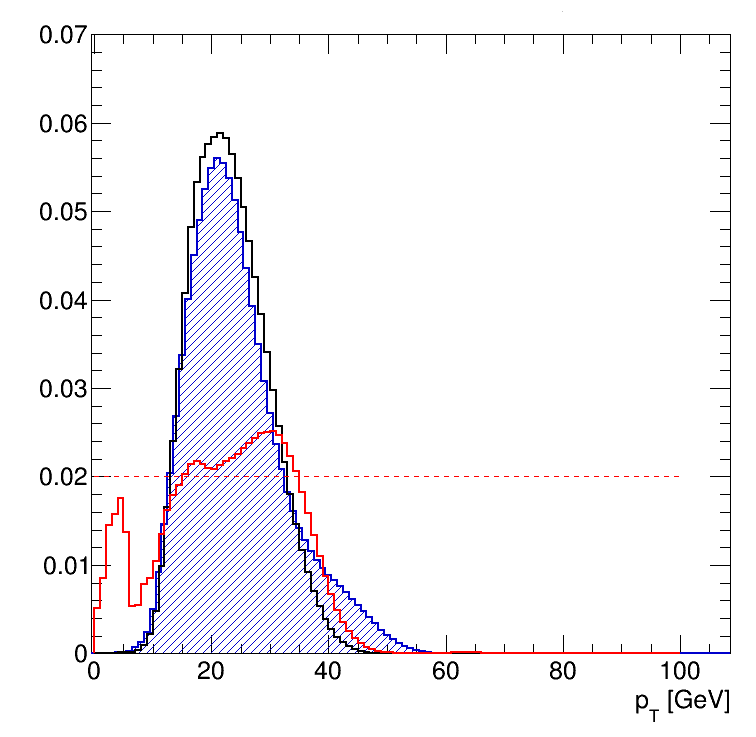
\includegraphics[width=0.49\textwidth]{figures/data_mc_samps/Pu-reweight2.png}
%     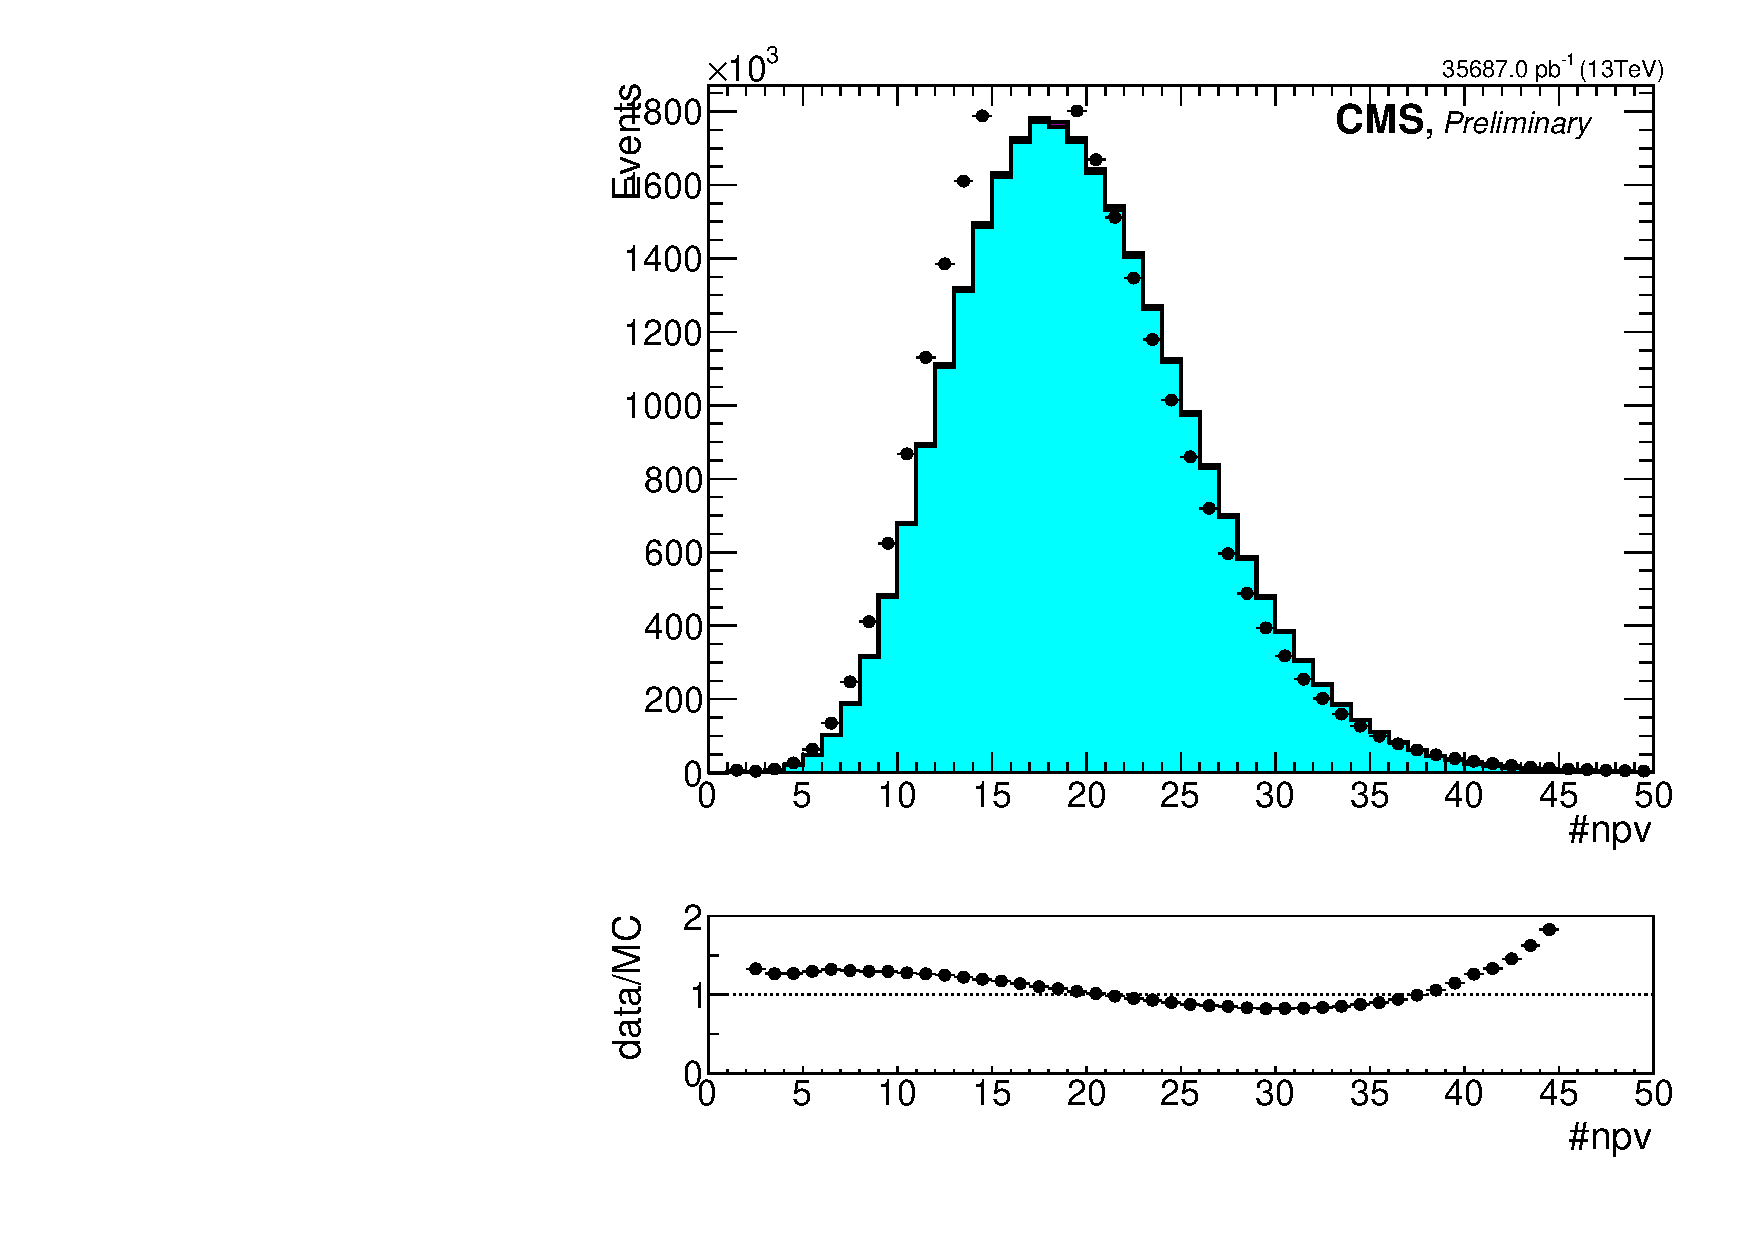
\includegraphics[width=0.49\textwidth]{figures/data_mc_samps/mmNpv_pileup69200.pdf}\\
%     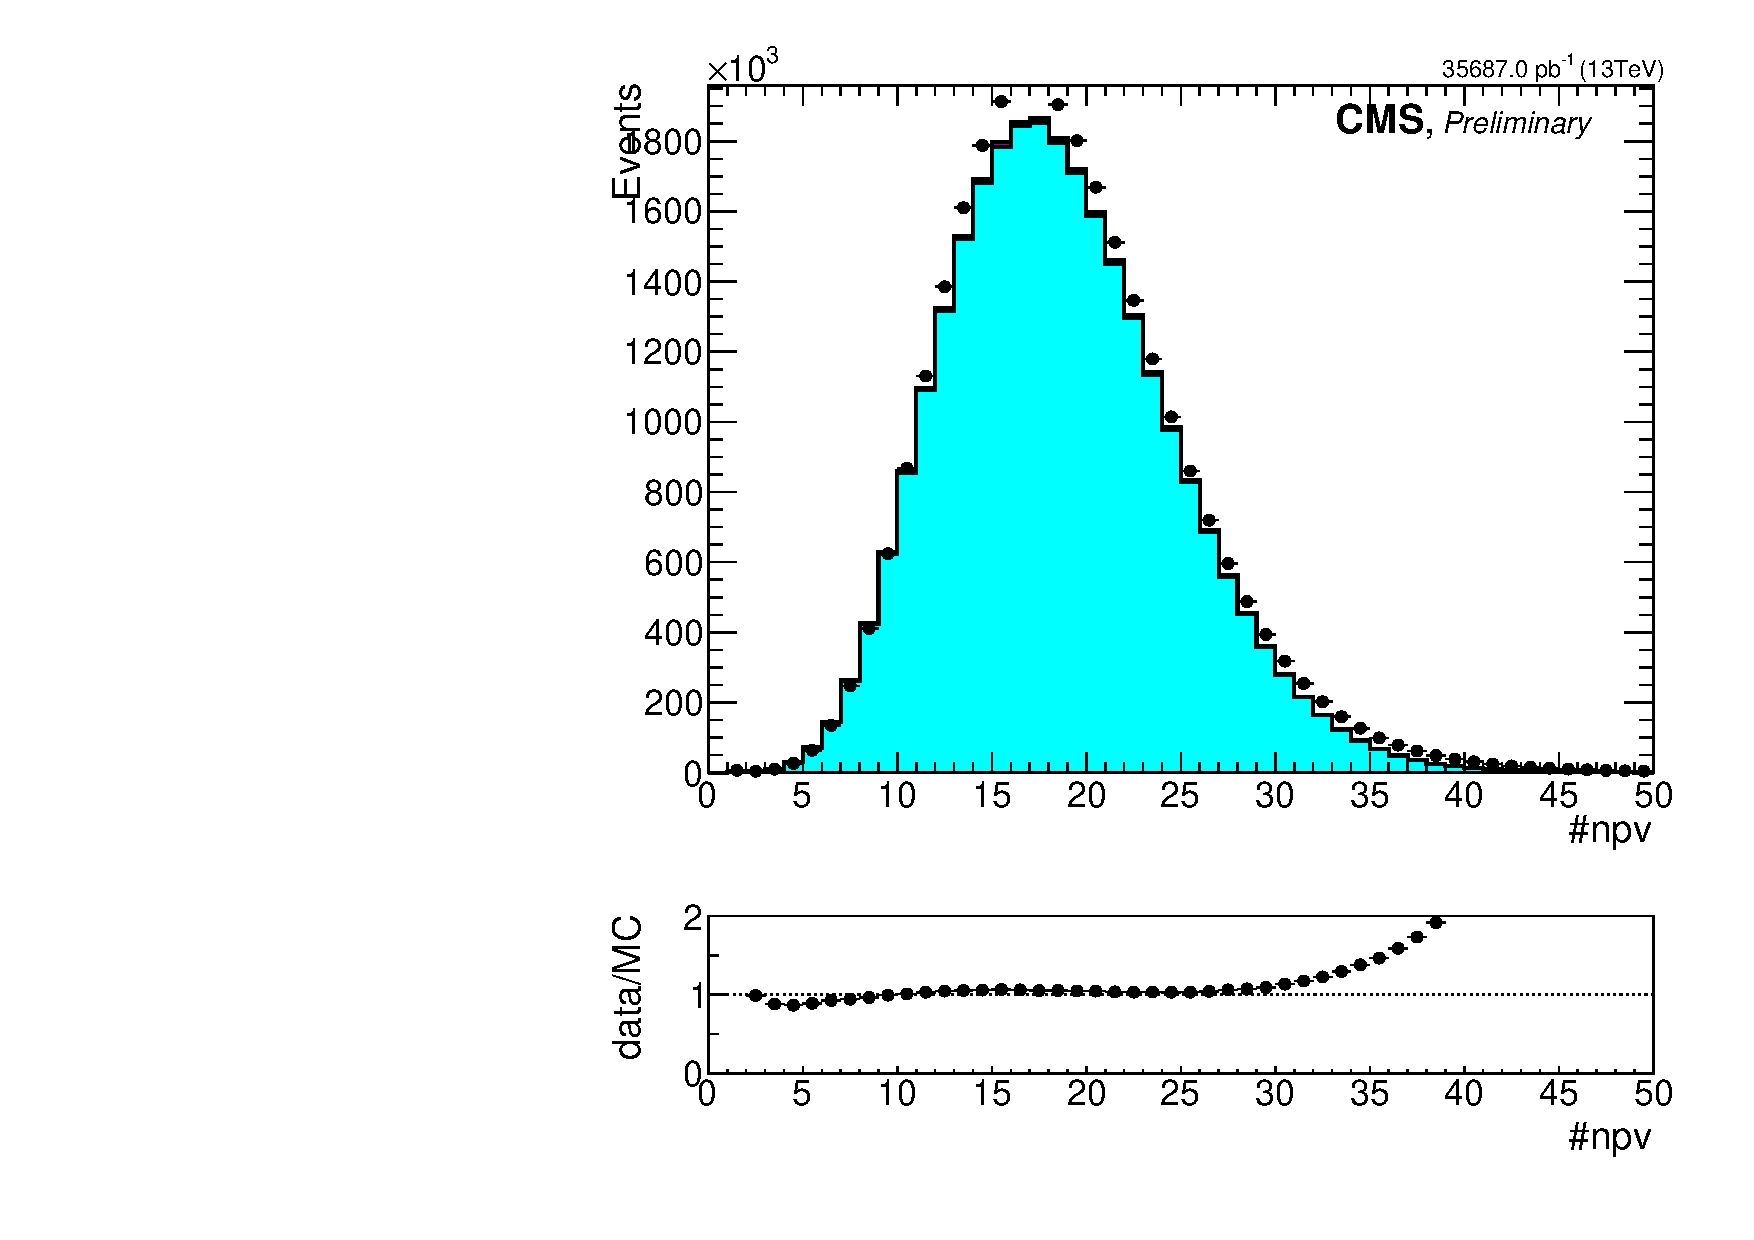
\includegraphics[width=0.49\textwidth]{figures/data_mc_samps/mmNpv_pileup65000.pdf}
%     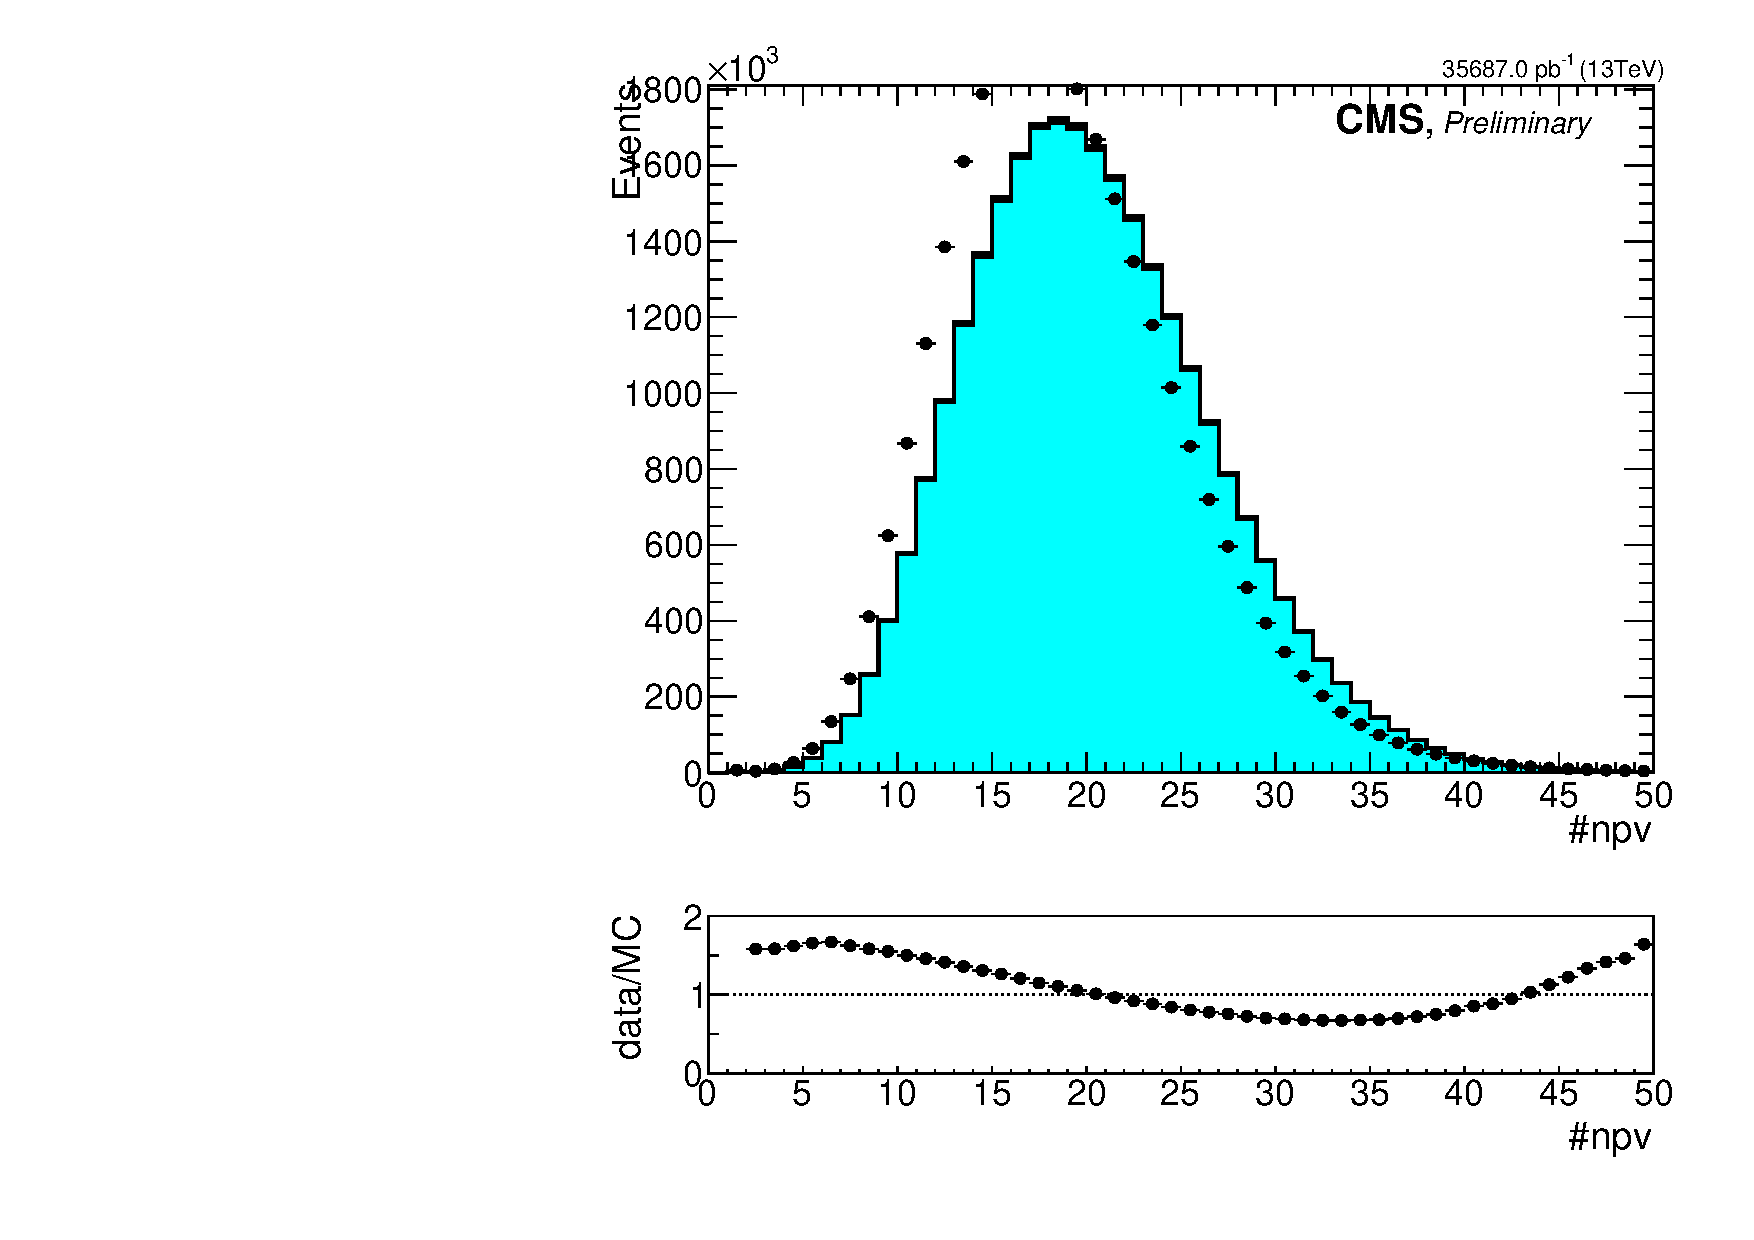
\includegraphics[width=0.49\textwidth]{figures/data_mc_samps/mmNpv_pileup72000.pdf}
%     \caption{Top Left. Pileup reweighting factors, data and MC truth pileup distributions. Top Right. agreement in the number of primary vertex variable after pu-reweighting. Bottom. agreement for the n.p.v. variables after $\pm1\sigma$ uncertainty in the pu-reweighting cress section.}
% \end{figure}



